%% Ternary complex model source
%% FigTCM.tex
%% Unused packages and definitions removed; TikZ/PGFPlots source formatted.

\documentclass{standalone}

\usepackage{tikz}
\usetikzlibrary{arrows}

\def\KG{K_G}
\def\KL{K_L}
\def\L{{\rm L}}
\def\G{{\rm G}}
\def\R{{\rm R}}
\def\LR{{\rm L}{\rm R}}
\def\RG{{\rm R}{\rm G}}
\def\LRG{{\rm L}{\rm R}{\rm G}}

\begin{document}

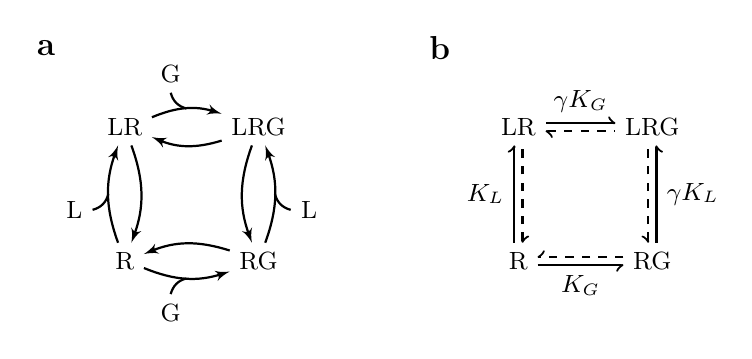
\begin{tikzpicture}[node distance=1.7cm,>=latex',font=\small]
    \begin{scope}[xshift=0cm]
        \node (LR) {$\LR$};
        \node[below of=LR] (R) {$\R$};
        \draw[->,thick] (LR) [bend left=20] to node[below] (firstmidwayabove) {} (R);
        \draw[->,thick] (R) to [bend left=20] node[above] (firstmidwaybelow) {} (LR);
        \draw[thick] (firstmidwaybelow.south) to [bend left] +(-0.2,-0.2) node[left] {$\L$};

        \node[right of=R] (RG) {$\RG$};
        \draw[<-,thick] (R) [bend left=20] to node[below] {} node[above] (firstmidwayabove) {} (RG);
        \draw[<-,thick] (RG) to [bend left=20] node[below] (firstmidwaybelow) {} (R);
        \draw[thick] (firstmidwaybelow.north) to [bend right] +(-0.2,-0.2) node[below] {$\G$};

        \node[right of=LR] (LRG) {$\LRG$};
        \draw[<-,thick] (RG) [bend left=20] to node[below] {} node[above] (firstmidwayabove) {} (LRG);
        \draw[<-,thick] (LRG) to [bend left=20] node[below] (firstmidwaybelow) {} (RG);
        \draw[thick] (firstmidwaybelow.north) to [bend right] +(0.2,-0.2) node[right] {$\L$};

        \draw[->,thick] (LR) [bend left=20] to node[below] {} node[above] (firstmidwayabove) {} (LRG);
        \draw[->,thick] (LRG) to [bend left=20] node[below] (firstmidwaybelow) {} (LR);
        \draw[thick] (firstmidwayabove.south) to [bend left] +(-0.2,0.2) node[above] {$\G$};

        \def\height{1}
        \def\left{-1}
        \draw (\left,\height) node[font=\large] {{\bf a}};
    \end{scope}

    \begin{scope}[xshift=5cm,yshift=0cm]
        \node (LR) {$\LR$};
        \node[below of=LR] (R) {$\R$};
        \draw[left to-,thick,transform canvas={xshift=-1.5pt}] (LR) to node[left] {$\KL$} (R);
        \draw[dashed,left to-,thick,transform canvas={xshift=1.5pt}] (R) to (LR);

        \node[right of=R] (RG) {$\RG$};
        \draw[-right to,thick,transform canvas={yshift=-1.5pt}] (R) to node[below] {$\KG$} (RG);
        \draw[dashed,-right to,thick,transform canvas={yshift=1.5pt}] (RG) to (R);

        \node[right of=LR] (LRG) {$\LRG$};
        \draw[dashed,right to-,thick,transform canvas={xshift=-1.5pt}] (RG) to (LRG);
        \draw[right to-,thick,transform canvas={xshift=1.5pt}] (LRG) to node[right] {$\gamma \KL$} (RG);
        \draw[dashed,left to-,thick,transform canvas={yshift=-1.5pt}] (LR) to (LRG);
        \draw[left to-,thick,transform canvas={yshift=1.5pt}] (LRG) to node[above] {$\gamma \KG$} (LR);

        \def\height{1}
        \def\left{-1}
        \draw (\left,\height) node[font=\large] {{\bf b}};
    \end{scope}

\end{tikzpicture}

\end{document}

